\chapter{Marco Teórico} \label{chapter:II}
\begin{spacing}{1.5}
\section{Open Source}
		Traducito literalemte como "fuente abierta", refiri\'{e}ndose as\'{i} a una caracter\'{i}stica del software donde el c\'{o}digo fuente es de libre acceso, sin embargo, Open Source no solo significa eso. Los t\'{e}rminos de distribuci\'{o}n de un software Open Source deben cumplir con los siguientes criterios:

		\begin{enumerate}
			\item \textbf{Distribuci\'{o}n gratuita}\\
			La licencia no impedirá a ninguna parte vender o regalar el software como un componente de una distribución de software agregada que contenga programas de varias fuentes diferentes. La licencia no requerirá regalías u otros honorarios por dicha venta \cite{chap2_open_source}.
			
			\item \textbf{C\'{o}digo fuente}\\
			El programa debe incluir el código fuente y debe permitir la distribución en código fuente y en forma compilada. Cuando alguna forma de un producto no se distribuye con el código fuente, debe haber un medio que est\'{e} bien publicitado para obtener el código fuente por un costo de reproducción no superior al razonable, preferiblemente, descargarlo a través de Internet sin cargo. El código fuente debe ser la forma preferida en la que un programador modificaría el programa. No se permite el código fuente deliberadamente ofuscado. No se permiten formas intermedias como la salida de un preprocesador o traductor \cite{chap2_open_source}.

			\item \textbf{Trabajos derivados}\\
			La licencia debe permitir modificaciones y trabajos derivados, y debe permitir que se distribuyan en los mismos términos que la licencia del software original \cite{chap2_open_source}.
			
			\item \textbf{Integridad del autor del c\'{o}digo fuente}\\
			La licencia puede restringir la distribución del código fuente en forma modificada solo si la licencia permite la distribución de "archivos de parche" con el código fuente con el fin de modificar el programa en el momento de la compilación. La licencia debe permitir explícitamente la distribución de software creado a partir del código fuente modificado. La licencia puede requerir que las obras derivadas lleven un nombre o número de versión diferente al del software original \cite{chap2_open_source}.
			
			\item \textbf{No discriminaci\'{o}n contra persona y grupos}\\
			La licencia no debe discriminar a ninguna persona o grupo de personas \cite{chap2_open_source}.
			
			\item \textbf{No discrininaci\'{o}n en los lugares de actividad}\\
			La licencia no debe restringir a nadie el uso del programa en un campo específico de actividad. Por ejemplo, no puede restringir el uso del programa en una empresa o para la investigación genética \cite{chap2_open_source}.
			
			\item \textbf{Licencia de distribuci\'{o}n}\\
			Los derechos adjuntos al programa deben aplicarse a todos aquellos a quienes se redistribuye el programa sin la necesidad de que esas partes ejecuten una licencia adicional \cite{chap2_open_source}.
			
			\item \textbf{La licencia no debe ser espec\'{i}fica para un producto}\\
			Los derechos adjuntos al programa no deben depender de que el programa sea parte de una distribución de software en particular. Si el programa se extrae de esa distribución y se usa o distribuye dentro de los términos de la licencia del programa, todas las partes a quienes se redistribuye el programa deben tener los mismos derechos que los que se otorgan junto con la distribución original del software \cite{chap2_open_source}.
			
			\item \textbf{La licencia no debe restringir a otro software}\\
			La licencia no debe imponer restricciones a otro software que se distribuya junto con el software con licencia. Por ejemplo, la licencia no debe insistir en que todos los demás programas distribuidos en el mismo medio deben ser software de código abierto \cite{chap2_open_source}.
			
			\item \textbf{La licencia debe ser de tecnología neutral}\\
			Ninguna disposición de la licencia puede basarse en una tecnología individual o estilo de interfaz \cite{chap2_open_source}.
			
		\end{enumerate}
	
\section{Legalidad del software}
	\subsection{Licencia}
	Una licencia es la autorización que se concede para explotar con fines industriales o comerciales una patente, marca o derecho. Diccionario de la lengua española (23.ª ed.)
	
	\subsection{Derecho de autor o Copyright}
	Derecho que la ley reconoce al autor de una obra intelectual o artística para autorizar su reproducción y participar en los beneficios que esta genere. Diccionario de la lengua española (23.ª ed.)
	
	\subsection{Patente}
	Documento expedido por una autoridad en que se acredita una condición o un mérito o se da la autorización para hacer algo. Diccionario de la lengua española (23.ª ed.)
	
	\subsection{Licencia de Software}
	Una licencia de software es un contrato entre el licenciante (autor/titular de los derechos de explotación/distribución) y el licenciatario (usuario consumidor, profesional o empresa) del programa informático, para utilizarlo cumpliendo una serie de términos y condiciones establecidas dentro de sus cláusulas, es decir, es un conjunto de permisos que un licenciante otorga a un usuario en los que tiene la posibilidad de distribuir, usar o modificar el producto bajo una licencia determinada. Además se suelen definir los plazos de duración, el territorio donde se aplica la licencia (ya que la licencia se soporta en las leyes particulares de cada país o región), entre otros.
	
	\subsection{Licencia Open Source}
	Las licencias de código abierto son licencias que cumplen con la definición de código abierto; en resumen, permiten que el software se utilice, modifique y comparta libremente. Para ser aprobada por Open Source Initiative (también conocida como OSI), una licencia debe pasar por el proceso de revisión de licencias de Open Source Initiative.\cite{chap2_open_source_2}\\
	
	Existen 100 licencias registradas en la Open Source Initiative(OSI), de las cual el presente proyecto describi\'{a} 2 de ellas por ser las m\'{a}s importante del proyecto Saiku Analytics.

	\subsubsection{Licencia Apache}
	La licencia de Apache solo requiere un reconocimiento en la ``documentación del usuario final" o ``en el software mismo", no en ``todos los materiales publicitarios". La licencia de Apache no especifica la prominencia que debe darse a ese reconocimiento. La licencia de Apache es consistente con los Principios de código abierto porque no interfiere con la libertad de modificar o crear trabajos derivados de software de código abierto.\cite{chap2_apache_license}\\
	Se deben añadir dos archivos en el directorio principal de los paquetes de software redistribuidos.
	\begin{enumerate}
		\item LICENSE: Una copia de la licencia
		\item NOTICE: Un documento de texto que incluye los “avisos” obligatorios del software presente en la distribución y una copia legible de estas notificaciones deben ser distribuidas como parte de los trabajos derivados, dentro de la forma de código fuente o documentación, o dentro de una pantalla generada por las obras derivadas ( donde aparecen normalmente este tipo de notificaciones a terceros).
	\end{enumerate}			

	\subsubsection{Licencia MIT}
	Licencia creada por los abogados del Instituto de Tecnología de Massachusetts (MIT) a partir de la licencia BSD. Limpiaron algo del lenguaje vago de la licencia BSD y facilitaron la lectura y la comprensión de su versión. En los Apéndices se muestra una copia de la versión actual de la licencia MIT.\\
	La concesión de la licencia del MIT se extiende no solo al software en sí, sino a sus archivos de documentación asociados. No está claro si el MIT se ofrece aquí para proporcionar toda la documentación en su poder sobre el software o solo ciertos archivos que están asociados de alguna manera con el software.\\
	La frase sin cargo significa que el licenciante (MIT en este caso) no cobrará regalías o derechos de licencia. Pero la palabra vender entre la lista de derechos otorgados significa que los licenciatarios posteriores no están restringidos de ninguna manera para cobrar regalías o tarifas de licencia a sus clientes por versiones modificadas del software.\\
	La licencia del MIT también sirve como plantilla de licencia. Es una licencia tan corta que solo es necesario cambiar el aviso de derechos de autor para completar la plantilla. Desafortunadamente, la frase este software y los archivos de documentación asociados no identifican claramente a qué software se aplica la licencia. La única forma de correlacionar un software en particular con una copia particular de la licencia del MIT es encontrar físicamente el texto de la licencia en el código fuente del software.\cite{chap2_MIT_license}\\
	
%------------------------------------------------------------------------------------------------------------------
%------------------------------------- Saiku Analytics ------------------------------------------------------------
%------------------------------------------------------------------------------------------------------------------	
\section{Saiku Analytics}
	Saiku fue fundada en 2008 por Tom Barber y Paul Stoellberger. Originalmente llamada \textit{Pentaho Analysis Tool}, comenzó como un contenedor básico basado en GWT alrededor de la biblioteca OLAP4J. A lo largo de los años ha evolucionado, y después de una reescritura completa en 2010, renació como Saiku.
	
	Saiku ofrece una solución de análisis basada en web fácil de usar que permite a los usuarios analizar rápida y fácilmente los datos corporativos y crear y compartir informes. La solución se conecta a una variedad de servidores OLAP, incluidos Mondrian, Microsoft Analysis Services, SAP BW y Oracle Hyperion y se puede implementar de manera rápida y rentable para permitir a los usuarios explorar datos en tiempo real.
	
	Saiku es una popular herramienta de análisis gráfico de código abierto para Mondrian que se puede ejecutar de forma independiente o como un complemento de Pentaho \cite{chap2_mondrian_action}.
	
	\subsection{Pentaho}
	Son una plataforma integral que se utilizan para acceder, integrar, manipular, visualizar y analizar datos. Ya sea que los datos se almacenen en un archivo plano, una base de datos relacional, un clúster Hadoop, una base de datos NoSQL, una base de datos analítica, transmisiones de redes sociales, tiendas operativas o en la nube, los productos Pentaho pueden ayudarlo a descubrir, analizar y visualizar datos para encontrar las respuestas que necesita, incluso si no tiene experiencia en codificación. Los usuarios avanzados con experiencia en programación pueden utilizar la extensa API para personalizar informes, consultas y transformaciones para ampliar la funcionalidad.\\
	Los productos de Pentaho incluyen tanto componentes basados en web como herramientas de diseño. Los componentes y herramientas que utiliza dependen de su flujo de trabajo y de lo que admita su entorno \cite{chap2_pentaho}.
	\subsubsection{Web-based Components}
	Son componentes basados en la web de Pentaho creados para compartir soluciones de inteligencia empresarial mediante el a\'{a}lisis de datos la creaci\'{o}n de informes y de paneles integrados.
		\begin{enumerate}[label=\alph*)]
			\item \textbf{Consola de usuario}\\
			La Consola de usuario de Pentaho (PUC) es un entorno de diseño para acceder a Analyzer, Reportes interactivos y Dashboard Designer. La consola de usuario de Pentaho también ofrece funciones de administración del sistema para configurar su servidor Pentaho \cite{chap2_pentaho}.
			
			\item \textbf{Analizador}\\
			Analyzer lo ayuda a visualizar datos para tomar decisiones comerciales informadas. Puede crear visualizaciones geográficas, gráficas de dispersión, cuadrículas térmicas y de múltiples gráficas. También puede filtrar datos, agregar parámetros de consulta, configurar enlaces detallados, aplicar formato condicional y generar hipervínculos \cite{chap2_pentaho}.
			
			\item \textbf{Informes interactivos}\\
			Interactive Reports es una interfaz de diseño que se utiliza para crear informes operativos simples y bajo demanda sin depender de TI o desarrolladores de informes. Puede agregar elementos rápidamente a su informe y aplicarles el formato que desee \cite{chap2_pentaho}.
			
			\item \textbf{Diseñador de paneles}\\
			Dashboard Designer se utiliza para elegir plantillas de diseño, temas y contenido para crear paneles visualmente atractivos que ayuden a los tomadores de decisiones a obtener conocimientos críticos de un vistazo. Puede combinar una amplia variedad de contenido, incluidos informes interactivos, visualizaciones del analizador y contenido colaborativo \cite{chap2_pentaho}.
			
			\item \textbf{CTools}\\
			CTools es un marco impulsado por la comunidad para crear paneles mediante el uso de tecnologías web como JavaScript, CSS y HTML. Puede crear fácilmente cuadros de mando dinámicos para que los usuarios exploren y comprendan grandes cantidades de datos mediante una variedad de gráficos, tablas y otros componentes \cite{chap2_pentaho}.
			
			\item \textbf{Asistente de fuente de datos}\\
			El Asistente de fuente de datos lo ayuda a definir una fuente de datos que contiene su información y lo guía a través de la creación de sus primeros modelos relacionales o multidimensionales para usar en la creación de informes y análisis \cite{chap2_pentaho}.
			
			\item \textbf{Editor de modelos de fuente de datos}\\
			El Editor de modelos de origen de datos le ayuda a ajustar y perfeccionar los modelos de datos relacionales y multidimensionales. Puede arrastrar campos a sus ubicaciones apropiadas, mezclar y combinar campos de diferentes tablas, agregar campos a más de una categoría o eliminar un campo \cite{chap2_pentaho}.
		\end{enumerate}
	\subsubsection{Design Tools}
	Las herramientas de diseño de Pentaho son para desarrollar y perfeccionar cómo se informan, modelan, transforman y almacenan los valores de sus datos.
		\begin{enumerate}
			\item \textbf{Integración de datos}\\
			Pentaho Data Integration (PDI) brinda acceso a un motor de extracción, transformación y carga (ETL) que captura los datos correctos, los limpia y los almacena utilizando un formato uniforme que es accesible y relevante para los usuarios finales y las tecnologías de IoT \cite{chap2_pentaho}.
			
			\item \textbf{Diseñador de informes}\\
			Report Designer se utiliza para generar informes detallados con píxeles perfectos utilizando prácticamente cualquier fuente de datos. Permite a los profesionales de inteligencia empresarial crear informes de calidad de impresi\'{o}n altamente detallados y basados en datos preparados adecuadamente \cite{chap2_pentaho}.
		
			\item \textbf{Diseñador de agregaciones}\\
			Aggregation Designer proporciona una interfaz simple que le permite crear tablas agregadas a partir de niveles dentro de las dimensiones que especifique. Utilice esta herramienta para mejorar el rendimiento de sus cubos OLAP de Pentaho Analysis (Mondrian) \cite{chap2_pentaho}.
			
			\item \textbf{Editor de metadatos}\\
			Metadata Editor simplifica la creación de informes. Utilice el editor de metadatos para crear modelos y dominios de metadatos de Pentaho. Un modelo de metadatos de Pentaho mapea la estructura física de su base de datos en un modelo de negocio lógico \cite{chap2_pentaho}.
			
			\item \textbf{Schema Workbench}\\
			Schema Workbench le permite editar y crear modelos multidimensionales (Mondrian). Puede crear modelos de Mondrian gráficamente o definirlos codificando manualmente archivos XML \cite{chap2_pentaho}.
		\end{enumerate}
%------------------------------------------------------------------------------------------------------------------
%-------------------------------------  SCRUM  --------------------------------------------------------------------
%------------------------------------------------------------------------------------------------------------------
\section{SCRUM}
	\subsection{Definici\'{o}n de Scrum}
		Scrum es un marco de trabajo liviano que ayuda a las personas, equipos y organizaciones a generar valor
		a través de soluciones adaptativas para problemas complejos \cite{chap2_scrum}.\\
		El marco de trabajo Scrum es incompleto de manera intencional, solo define las
		partes necesarias para implementar la teoría de Scrum. Scrum se basa en la inteligencia colectiva de las
		personas que lo utilizan. En lugar de proporcionar a las personas instrucciones detalladas, las reglas de
		Scrum guían sus relaciones e interacciones.\\
		En este marco de trabajo pueden emplearse varios procesos, técnicas y métodos. Scrum envuelve las
		prácticas existentes o las hace innecesarias. Scrum hace visible la eficacia relativa de las técnicas
		actuales de gestión, entorno y trabajo, de modo que se puedan realizar mejoras.
	\subsection{Teor\'{i}a de Scrum}
		Scrum se basa en el empirismo y el pensamiento Lean. El empirismo afirma que el conocimiento
		proviene de la experiencia y de la toma de decisiones con base en lo observado. El pensamiento Lean
		reduce el desperdicio y se enfoca en lo esencial.\\
		Scrum emplea un enfoque iterativo e Incremental para optimizar la previsibilidad y controlar el riesgo.
		Scrum involucra a grupos de personas que colectivamente tienen todas las habilidades y experiencia
		para hacer el trabajo y compartir o adquirir dichas habilidades según sea necesario.
		Scrum combina cuatro eventos formales para inspección y adaptación dentro de un evento contenedor,
		el Sprint. Estos eventos funcionan porque implementan los pilares empíricos de Scrum de transparencia,
		inspección y adaptación \cite{chap2_scrum}.
		\subsubsection{Transparencia}
			El proceso y el trabajo emergentes deben ser visibles tanto para quienes realizan el trabajo como para
			quienes lo reciben. Con Scrum, las decisiones importantes se basan en el estado percibido de sus tres artefactos formales. Los artefactos que tienen poca transparencia pueden llevar a decisiones que
			disminuyan el valor y aumenten el riesgo.\\
			La transparencia permite la inspección. La inspección sin transparencia es engañosa y derrochadora \cite{chap2_scrum}.
		\subsubsection{Inspecci\'{o}n}
			Los artefactos de Scrum y el progreso hacia los objetivos acordados deben inspeccionarse con
			frecuencia y con diligencia para detectar variaciones o problemas potencialmente indeseables. Para
			ayudar con la inspección, Scrum proporciona cadencia en forma de sus cinco eventos.\\
			La inspección permite la adaptación. La inspección sin adaptación se considera inútil. Los eventos Scrum
			están diseñados para provocar cambios \cite{chap2_scrum}.
		\subsubsection{Adaptaci\'{o}n}
			Si algún aspecto de un proceso se desvía fuera de los límites aceptables o si el producto resultante es
			inaceptable, el proceso que se aplica o los materiales que se producen deben ajustarse. El ajuste debe
			realizarse lo antes posible para minimizar una mayor desviación.\\
			La adaptación se vuelve más difícil cuando las personas involucradas no están empoderadas ni se
			autogestionan. Se espera que un Scrum Team se adapte en el momento en que aprenda algo nuevo a
			través de la inspección \cite{chap2_scrum}.
	\subsection{Valores de Scrum}
			El uso exitoso de Scrum depende de que las personas se vuelvan más competentes en vivir cinco valores: \textbf{Compromiso, Foco, Franqueza, Respeto y Coraje}.
			El Scrum Team se compromete a lograr sus objetivos y a apoyarse mutuamente. Su foco principal está
			en el trabajo del Sprint para lograr el mejor progreso posible hacia estos objetivos. El Scrum Team y sus interesados son francos sobre el trabajo y los desafíos. Los miembros del Scrum Team se respetan entre sí para ser personas capaces e independientes, y son respetados como tales por las personas con las que	trabajan. Los miembros del Scrum Team tienen el coraje de hacer lo correcto, para trabajar en
			problemas difíciles \cite{chap2_scrum}.\\
			Estos valores dan dirección al Scrum Team con respecto a su trabajo, acciones y comportamiento. Las
			decisiones que se tomen, los pasos que se den y la forma en que se use Scrum deben reforzar estos
			valores, no disminuirlos ni socavarlos. Los miembros del Scrum Team aprenden y exploran los valores
			mientras trabajan con los eventos y artefactos Scrum. Cuando el Scrum Team y las personas con las que trabajan incorporan estos valores, los pilares empíricos de Scrum de transparencia, inspección y 		adaptación cobran vida y generan confianza.
	\subsection{\textit{Scrum Team}}
		La unidad fundamental de Scrum es un pequeño equipo de personas, un \textit{Scrum Team}. El \textit{Scrum Team} consta de un \textit{Scrum Master}, un \textit{Product Owner} y \textit{Developers}. Dentro de un \textit{Scrum Team}, no hay subequipos ni jerarquías. Es una unidad cohesionada de profesionales enfocados en un objetivo a la vez, el Objetivo del Producto.
		Los \textit{Scrum Teams} son multifuncionales, lo que significa que los miembros tienen todas las habilidades
		necesarias para crear valor en cada \textit{Sprint}. También se autogestionan, lo que significa que deciden
		internamente quién hace qué, cuándo, cómo y porqu\'{e} \cite{chap2_scrum}.\\
		El \textit{Scrum Team} es lo suficientemente pequeño como para seguir siendo ágil y lo suficientemente grande
		como para completar un trabajo significativo dentro de un Sprint, generalmente 10 personas o menos.
		En general, hemos descubierto que los equipos más pequeños se comunican mejor y son más
		productivos. Si los \textit{Scrum Teams} se vuelven demasiado grandes, deberían considerar reorganizarse en
		múltiples \textit{Scrum Teams} cohesivos, cada uno enfocado en el mismo producto. Por lo tanto, deben
		compartir el mismo Objetivo del Producto, el \textit{Product Backlog} y el \textit{Product Owner}.
		El \textit{Scrum Team} es responsable de todas las actividades relacionadas con el producto, desde la
		colaboración de los interesados, la verificación, el mantenimiento, la operación, la experimentación, la
		investigación y el desarrollo, y cualquier otra cosa que pueda ser necesaria. Están estructurados y
		empoderados por la organización para gestionar su propio trabajo. Trabajar en \textit{Sprints} a un ritmo
		sostenible mejora el enfoque y la consistencia del \textit{Scrum Team} \cite{chap2_scrum}.
		Todo el Scrum Team es responsable de crear un Increment valioso y útil en cada Sprint. Scrum define
		tres responsabilidades específicas dentro del Scrum Team: los \textit{Developers}, el \textit{Product Owner} y el \textit{Scrum Master}.
		\subsubsection{Developers}
			Son Las personas del \textit{Scrum Team} que se comprometen a crear cualquier aspecto de un \textit{Increment} utilizable en cada \textit{Sprint} son \textit{Developers}.
			Las habilidades específicas que necesitan los \textit{Developers} suelen ser amplias y variarán según el ámbito
			de trabajo. Sin embargo, los \textit{Developers} siempre son responsables de:
			\begin{itemize}
				\item Crear un plan para el \textit{Sprint}, el \textit{Sprint Backlog};
				\item Inculcar calidad al adherirse a una Definición de Terminado;
				\item Adaptar su plan cada día hacia el Objetivo del \textit{Sprint}; y,
				\item Responsabilizarse mutuamente como profesionales.
			\end{itemize}
		\subsubsection{Product Owner}
			El \textit{Product Owner} es responsable de maximizar el valor del producto resultante del trabajo del \textit{Scrum Team}. La forma en que esto se hace puede variar ampliamente entre organizaciones, \textit{Scrum Teams} e individuos.\\
			El \textit{Product Owner} también es responsable de la gestión efectiva del \textit{Product Backlog}, lo que incluye:
			\begin{itemize}
				\item Desarrollar y comunicar explícitamente el Objetivo del Producto;
				\item Crear y comunicar claramente los elementos del \textit{Product Backlog};
				\item Ordenar los elementos del \textit{Product Backlog}; y,
				\item Asegurarse de que el \textit{Product Backlog} sea transparente, visible y se entienda.
			\end{itemize}
			El \textit{Product Owner} puede realizar el trabajo anterior o puede delegar la responsabilidad en otros. Independientemente de ello, el \textit{Product Owner} sigue siendo el responsable de que el trabajo se realice.\\
			Para que los \textit{Product Owners} tengan éxito, toda la organización debe respetar sus decisiones. Estas decisiones son visibles en el contenido y el orden del \textit{Product Backlog}, y a través del \textit{Increment} inspeccionable en la \textit{Sprint Review}.\\
			El \textit{Product Owner} es una persona, no un comité. El \textit{Product Owner} puede representar las necesidades de muchos interesados en el \textit{Product Backlog}. Aquellos que quieran cambiar el \textit{Product Backlog} pueden hacerlo intentando convencer al \textit{Product Owner}.
		\subsubsection{Scrum Master}
			El Scrum Master es responsable de establecer Scrum como se define en la Guía de Scrum. Lo hace ayudando a todos a comprender la teoría y la práctica de Scrum, tanto dentro del \textit{Scrum Team} como de la organización.\\
			El \textit{Scrum Master} es responsable de lograr la efectividad del \textit{Scrum Team}. Lo hace apoyando al \textit{Scrum Team} en la mejora de sus prácticas, dentro del marco de trabajo de Scrum.\\
			Los \textit{Scrum Masters} son verdaderos líderes que sirven al \textit{Scrum Team} y a la organización en general \cite{chap2_scrum}.\\
			El \textit{Scrum Master} sirve al \textit{Scrum Team} de varias maneras, que incluyen:
			\begin{itemize}
				\item Guiar a los miembros del equipo en ser autogestionados y multifuncionales;
				\item Ayudar al \textit{Scrum Team} a enfocarse en crear \textit{Increments} de alto valor que cumplan con la``Definición de Terminado";
				\item Procurar la eliminación de impedimentos para el progreso del \textit{Scrum Team}; y,
				\item Asegurarse de que todos los eventos de Scrum se lleven a cabo y sean positivos, productivos y se mantengan dentro de los límites de tiempo recomendados en la gu\'{i}a de Scrum.
			\end{itemize}
			El \textit{Scrum Master} sirve al \textit{Product Owner} de varias maneras, que incluyen:
			\begin{itemize}
				\item Ayudar a encontrar técnicas para una definición efectiva de Objetivos del Producto y la gestión	del \textit{Product Backlog};
				\item Ayudar al \textit{Scrum Team} a comprender la necesidad de tener elementos del \textit{Product Backlog} claros y concisos;
				\item Ayudar a establecer una planificación empírica de productos para un entorno complejo; y,
				\item Facilitar la colaboración de los interesados según se solicite o necesite.
			\end{itemize}
			El Scrum Master sirve a la organización de varias maneras, que incluyen:
			\begin{itemize}
			\item Liderar, capacitar y guiar a la organización en su adopción de Scrum;
			\item Planificar y asesorar implementaciones de Scrum dentro de la organización;
			\item Ayudar a los empleados y los interesados a comprender y aplicar un enfoque empírico para el trabajo complejo; y,
			\item Eliminar las barreras entre los interesados y los \textit{Scrum Teams}.
			\end{itemize}
	\subsection{Eventos de Scrum}
		El \textit{Sprint} es un contenedor para todos los demás eventos. Cada evento en Scrum es una oportunidad formal para inspeccionar y adaptar los artefactos Scrum. Estos eventos están diseñados específicamente para habilitar la transparencia requerida. No operar cualquier evento según lo prescrito resulta en la pérdida de oportunidades para inspeccionar y adaptarse. Los eventos se utilizan en Scrum para crear regularidad y minimizar la necesidad de reuniones no definidas en Scrum.\\
		Lo óptimo es que todos los eventos se celebren al mismo tiempo y en el mismo lugar para reducir la complejidad \cite{chap2_scrum}, los eventos se pueden apreciar detalladamente en la Figura \ref{figure:chaperII_1}.
		\begin{figure}[H]
			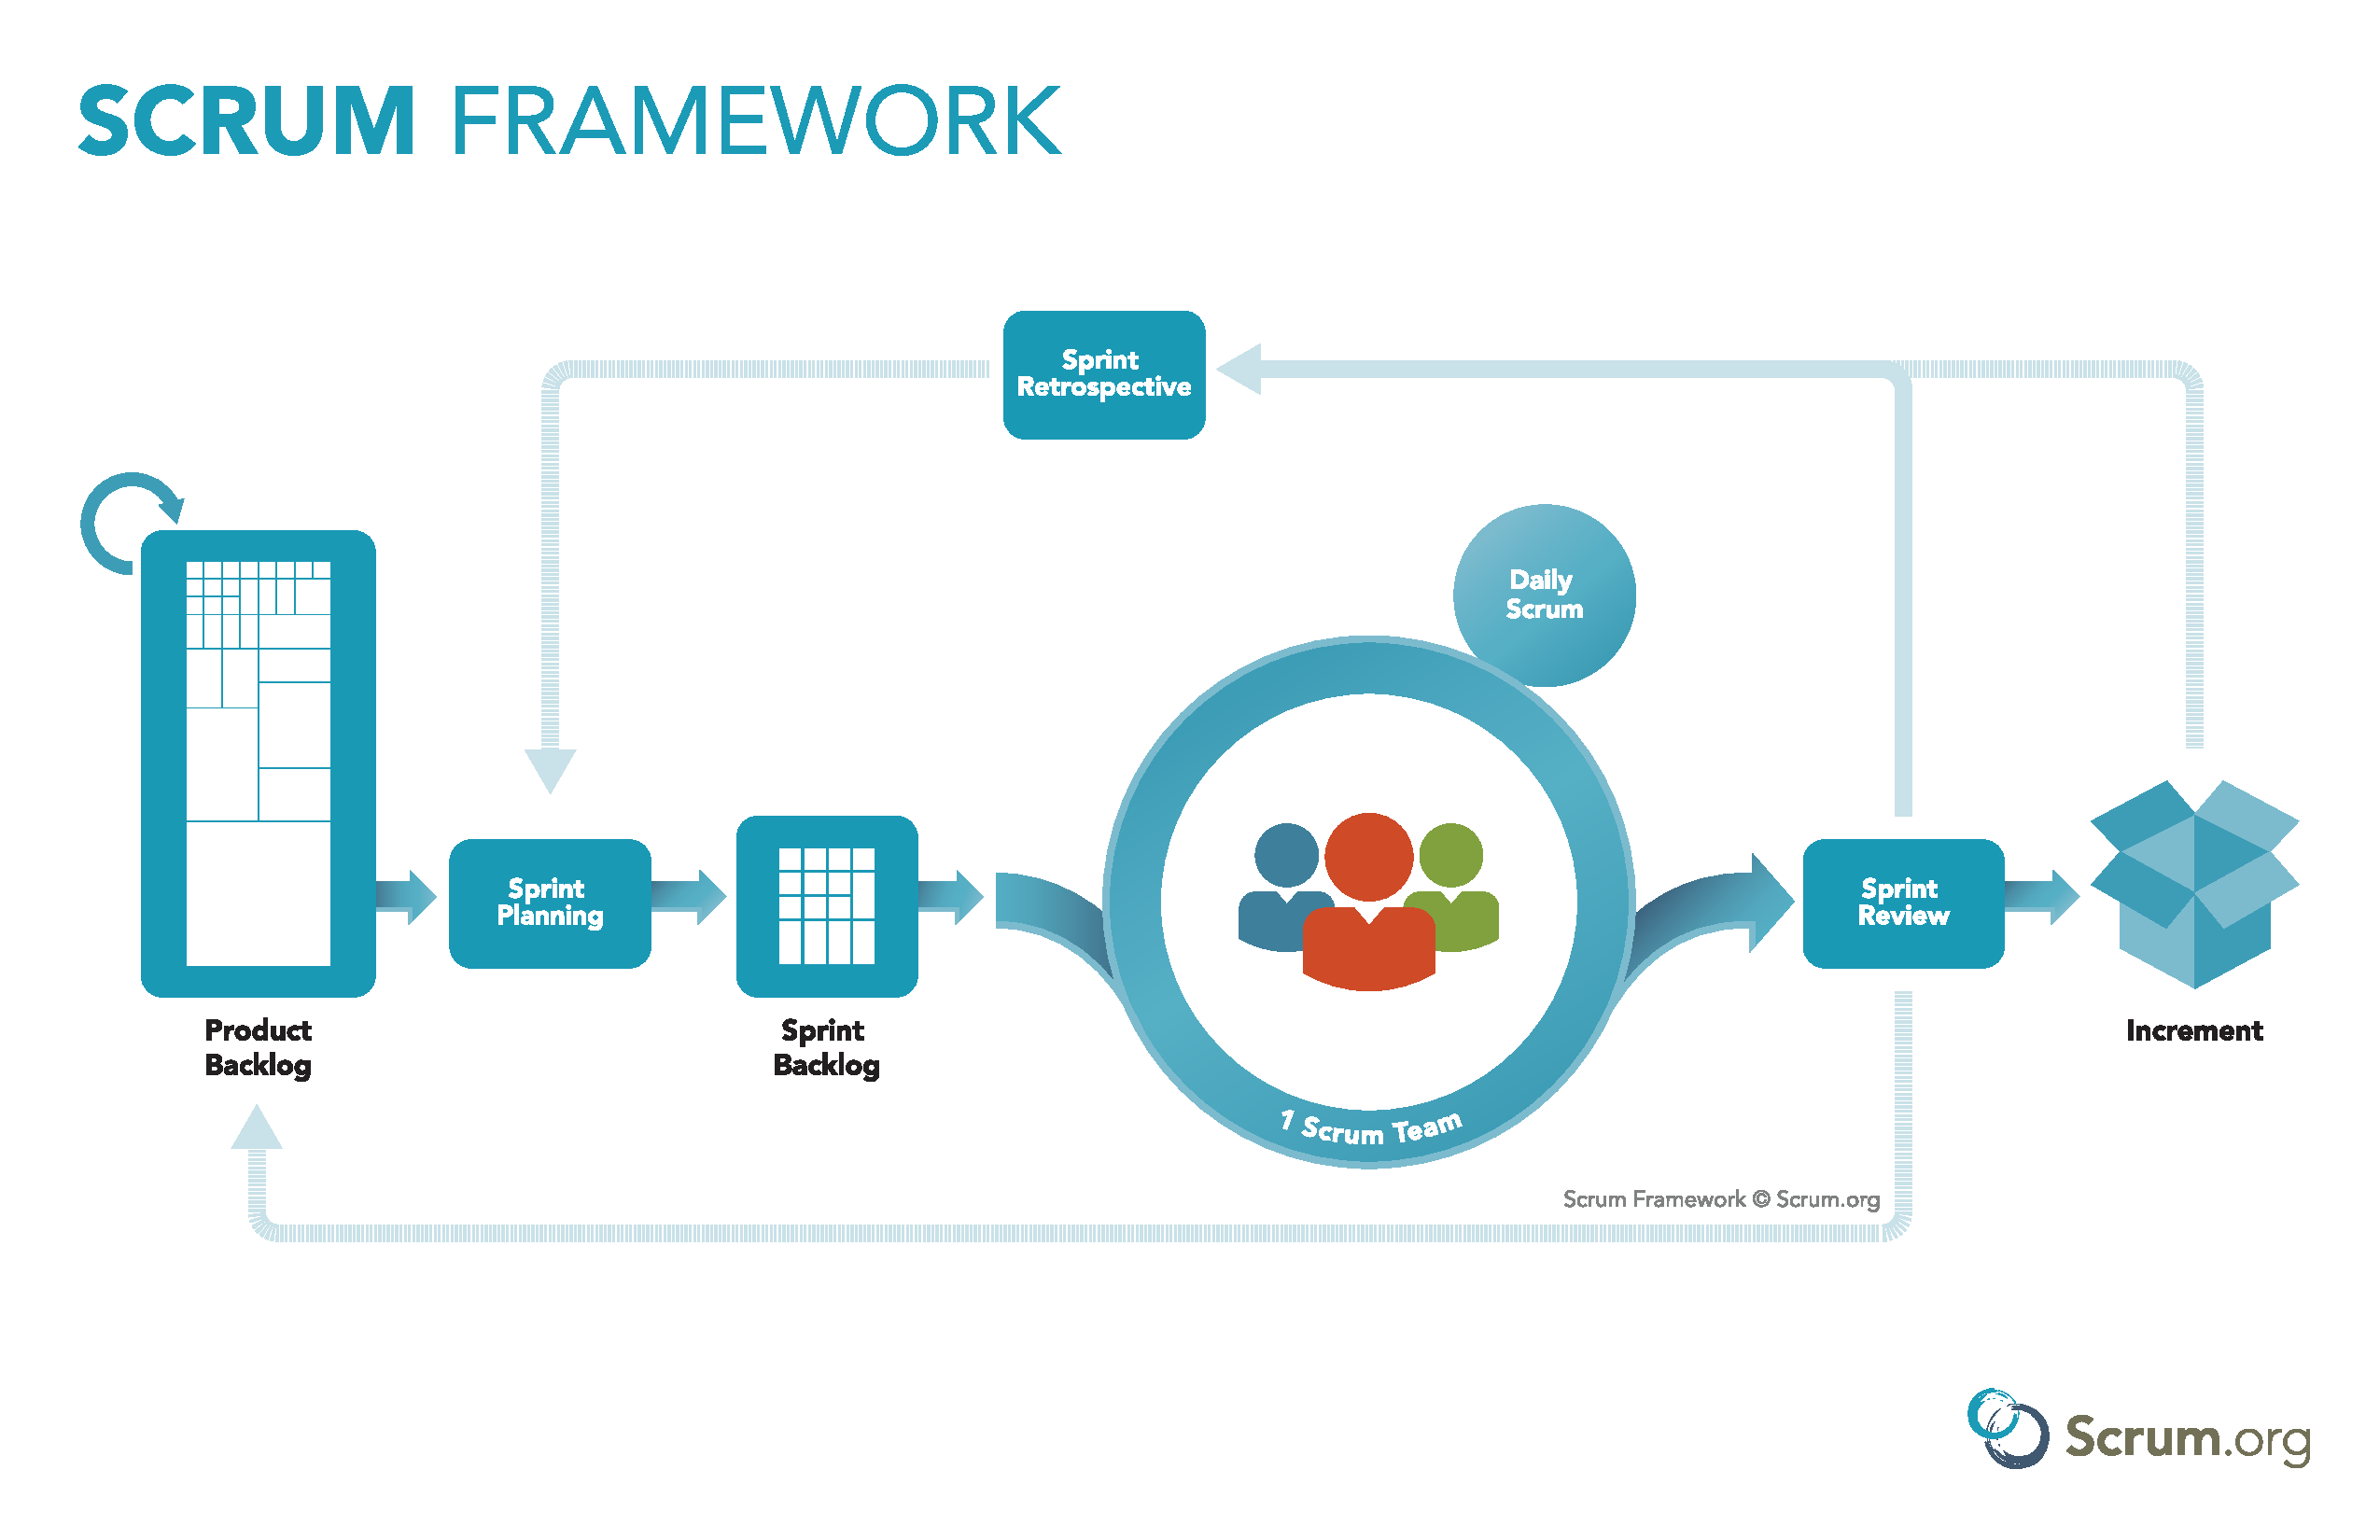
\includegraphics[page=1,width=1.0 \textwidth]{scrum.pdf}
			\caption {\centering \small{Scrum Framework} \\ hi}\label{figure:chaperII_1}
		\end{figure}
		\subsubsection{El \textit{Sprint}}
			Los Sprints son el corazón de Scrum, donde las ideas se convierten en valor.\\
			Son eventos de duración fija de un mes o menos para crear consistencia. Un nuevo Sprint comienza inmediatamente después de la conclusión del Sprint anterior.\\
			Todo el trabajo necesario para lograr el Objetivo del Producto, incluido la \textit{Sprint Planning}, \textit{Daily Scrums}, \textit{Sprint Review} y \textit{Sprint Retrospective}, ocurre dentro de los \textit{Sprints} \cite{chap2_scrum}.\\
			Durante el Sprint:
			\begin{itemize}
				\item No se realizan cambios que pongan en peligro el Objetivo del \textit{Sprint};
				\item La calidad no disminuye;
				\item El \textit{Product Backlog} se refina según sea necesario; y,
				\item El alcance se puede aclarar y renegociar con el \textit{Product Owner} a medida que se aprende más.
			\end{itemize}
			Los \textit{Sprints} permiten la previsibilidad al garantizar la inspección y adaptación del progreso hacia un Objetivo del Producto al menos cada mes calendario. Cuando el horizonte de un \textit{Sprint} es demasiado largo, el Objetivo del \textit{Sprint} puede volverse inválido, la complejidad puede crecer y el riesgo puede aumentar. Se pueden emplear \textit{Sprints} más cortos para generar más ciclos de aprendizaje y limitar el riesgo de costo y esfuerzo a un período de tiempo menor. Cada \textit{Sprint} puede considerarse un proyecto corto.\\
			Existen varias prácticas para pronosticar el progreso, como el trabajo pendiente (\textit{burn‐downs}), trabajo completado (\textit{burn‐ups}) o flujos acumulativos (\textit{cumulative flows}). Si bien han demostrado su utilidad, no reemplazan la importancia del empirismo. En entornos complejos, se desconoce lo que sucederá. Solo lo que ya ha sucedido se puede utilizar para la toma de decisiones con miras al futuro.\\
			Un \textit{Sprint} podría cancelarse si el Objetivo del \textit{Sprint} se vuelve obsoleto. Solo el \textit{Product Owner} tiene la autoridad para cancelar el \textit{Sprint}.
		\subsubsection{\textit{Sprint Planning}}
			La \textit{Sprint Planning} inicia el \textit{Sprint} al establecer el trabajo que se realizará para el \textit{Sprint}. El \textit{Scrum Team} crea este plan resultante mediante trabajo colaborativo.\\
			El \textit{Product Owner} se asegura de que los asistentes estén preparados para discutir los elementos más importantes del \textit{Product Backlog} y cómo se relacionan con el Objetivo del Producto. El \textit{Scrum Team} también puede invitar a otras personas a asistir a la \textit{Sprint Planning} para brindar asesoramiento \cite{chap2_scrum}.\\
			El \textit{Sprint Planning} aborda los siguientes temas:
			\begin{itemize}
				\item Tema uno: ¿Por qué es valioso este \textit{Sprint}?\\
				El \textit{Product Owner} propone cómo el producto podría \textit{Incrementar} su valor y utilidad en el \textit{Sprint} actual. Luego, todo el \textit{Scrum Team} colabora para definir un Objetivo del \textit{Sprint} que comunica por qué el \textit{Sprint} es valioso para los interesados. El Objetivo del \textit{Sprint} debe completarse antes de que termine la \textit{Sprint Planning}.
				\item Tema dos: ¿Qué se puede hacer en este \textit{Sprint}?\\
				A través de una conversación con el \textit{Product Owner}, los \textit{Developers} seleccionan elementos del \textit{Product Backlog} para incluirlos en el \textit{Sprint} actual. El \textit{Scrum Team} puede refinar estos elementos durante este proceso, lo que aumenta la comprensión y la confianza.\\
				Seleccionar cuánto se puede completar dentro de un \textit{Sprint} puede ser un desafío. Sin embargo, cuanto más sepan los \textit{Developers} sobre su desempeño pasado, su capacidad actual y su ``Definición de Terminado", más confiados estarán en sus pronósticos para el \textit{Sprint}.
				\item Tema tres: ¿Cómo se realizará el trabajo elegido?\\
				Para cada elemento del \textit{Product Backlog} seleccionado, los \textit{Developers} planifican el trabajo necesario para crear un \textit{Increment} que cumpla con la ``Definición de Terminado". A menudo, esto se hace descomponiendo los elementos del \textit{Product Backlog} en elementos de trabajo más pequeños de un día o menos. La forma de hacerlo queda a criterio exclusivo de los \textit{Developers}. Nadie más les dice cómo convertir los elementos del \textit{Product Backlog} en \textit{Increments} de valor.\\
				El Objetivo del \textit{Sprint}, los elementos del \textit{Product Backlog} seleccionados para el Sprint, más el plan para entregarlos se denominan juntos \textit{Sprint Backlog}.
				El \textit{Sprint Planning} tiene un límite de tiempo de máximo ocho horas para un \textit{Sprint} de un mes. Para \textit{Sprints} más cortos, el evento suele ser de menor duración.
			\end{itemize}
		\subsubsection{\textit{Daily Scrum}}
			El propósito del \textit{Daily Scrum} es inspeccionar el progreso hacia el Objetivo del \textit{Sprint} y adaptar el \textit{Sprint Backlog} según sea necesario, ajustando el trabajo planificado entrante. El Daily Scrum es un evento de 15 minutos para los \textit{Developers} del \textit{Scrum Team}. Para reducir la complejidad, se lleva a cabo a la misma hora y en el mismo lugar todos los días hábiles del \textit{Sprint}. Si el \textit{Product Owner} o \textit{Scrum Master} están trabajando activamente en elementos del \textit{Sprint Backlog}, participan como \textit{Developers} \cite{chap2_scrum}.
			Los \textit{Developers} pueden seleccionar la estructura y las técnicas que deseen, siempre que su \textit{Daily Scrum} se centre en el progreso hacia el Objetivo del \textit{Sprint} y produzca un plan viable para el siguiente día de trabajo. Esto crea enfoque y mejora la autogestión.\\
			Los \textit{Daily Scrums} mejoran la comunicación, identifican impedimentos, promueven la toma rápida de
			decisiones y, en consecuencia, eliminan la necesidad de otras reuniones.\\
			El \textit{Daily Scrum} no es el único momento en el que los \textit{Developers} pueden ajustar su plan. A menudo se reúnen durante el día para discusiones más detalladas sobre cómo adaptar o volver a planificar el resto del trabajo del \textit{Sprint}.
		\subsubsection{\textit{Sprint Review}}
			El propósito del \textit{Sprint Review} es inspeccionar el resultado del \textit{Sprint} y determinar futuras	adaptaciones. El \textit{Scrum Team} presenta los resultados de su trabajo a los interesados clave y se discute el progreso hacia el Objetivo del Producto.\\
			Durante el evento, el \textit{Scrum Team} y los interesados revisan lo que se logró en el Sprint y lo que ha cambiado en su entorno. Con base en esta información, los asistentes colaboran sobre qué hacer a
			continuación. El \textit{Product Backlog} también se puede ajustar para satisfacer nuevas oportunidades. El \textit{Sprint Review} es una sesión de trabajo y el \textit{Scrum Team} debe evitar limitarla a una presentación.\\
			La \textit{Sprint Review} es el penúltimo evento del \textit{Sprint} y tiene un límite de tiempo de máximo cuatro horas para un \textit{Sprint} de un mes. Para \textit{Sprints} más cortos, el evento suele ser de menor duración.
		\subsubsection{\textit{Sprint Retrospective}}
					\lipsum[1]
	\subsection{Artefactos de Scrum}
				\lipsum[1]
		\subsubsection{\textit{Product Backlog}}
					\lipsum[1]
		\subsubsection{\textit{Sprint Backlog}}
					\lipsum[1]
		\subsubsection{\textit{Increment}}
					\lipsum[1]
	\subsection{Cambios de la gu\'{i}a Scrum 2017 a la gu\'{i}a Scrum 2020}
				\lipsum[1]
%------------------------------------------------------------------------------------------------------------------	
%-----------------------------  Extreme Programming ---------------------------------------------------------------
%------------------------------------------------------------------------------------------------------------------
\section{Programaci\'{o}n Extrema(XP)}
		\lipsum[1-2]
	\subsection{Valores, Principios y Pr\'{a}cticas}
			\lipsum[1]
	\subsection{Valores}
				\lipsum[1]
	\subsection{Principios}
				\lipsum[1]
	\subsection{Pr\'{a}cticas}
				\lipsum[1]
		\subsubsection{Pr\'{a}cticas primarias}
					\lipsum[1]
		\subsubsection{Pr\'{a}cticas corolarias}
					\lipsum[1]
	\subsection{Planeaci\'{o}n}
				\lipsum[1]
	\subsection{Dise\'{n}o}
				\lipsum[1]
	\subsection{Pruebas}
				\lipsum[1]
%------------------------------------------------------------------------------------------------------------------
%-------------------------------Tecnologias backend para la integracion--------------------------------------------
%------------------------------------------------------------------------------------------------------------------
\section{Tecnolog\'{i}as BackEnd para la integraci\'{o} del proyecto Saiku Analytics}
		\lipsum[1-2]
	\subsection{Lenguaje de programaci\'{o}n Java}
			\lipsum[1-2]
	\subsection{Java Specification Requests(JSRs)}
		\subsubsection{JSR-366}
				\lipsum[1-2]
		\subsubsection{JSR-47}
				\lipsum[1-2]
		\subsubsection{JSR-338}
				\lipsum[1-2]
		\subsubsection{JSR-346}
				\lipsum[1-2]
		\subsubsection{JSR-369}
				\lipsum[1-2]
		\subsubsection{JSR-370}
		\lipsum[1-2]
		\subsubsection{JSR-371}
		\lipsum[1-2]
	\subsection{\textit{Spring Framework}}
			\lipsum[1-2]
		\subsubsection{\textit{Spring security}}
				\lipsum[1-2]
	\subsection{Maven}
			\lipsum[1-2]
	\subsection{Mondian}
			\lipsum[1-2]
	\subsection{Git}
			\lipsum[1-2]
	\subsection{Enunciate}
			\lipsum[1-2]
%------------------------------------------------------------------------------------------------------------------
%-------------------------------Tecnologias backend para la integracion--------------------------------------------
%------------------------------------------------------------------------------------------------------------------
\section{Tecnolog\'{i}as FrontEnd para la integraci\'{o}n
		 del proyecto Saiku Analytics}
		\lipsum[1-2]
	\subsection{ECMAScript6 (ES6)}
			\lipsum[1-2]
	\subsection{HTML5}
			\lipsum[1-2]
	\subsection{Javascript}
			\lipsum[1-2]
	\subsection{Css}
			\lipsum[1-2]
	\subsection{Backbone}
			\lipsum[1-2]
	\subsection{Node.js}
			\lipsum[1-2]
	\subsection{CCC-Charts}
			\lipsum[1-2]
\end{spacing}
		
		
		
%JCache (JSR-107)
%Java API for JSON Binding (JSR-367)
%Model View Controller (MVC) (JSR-371)
%Java API for WebSocket
%Java API for JSON Processing (JSON-P)
%Java API for RESTful Web Services (JAX-RS) JSR-370
%JavaServer Faces (JSF)
%Java Servlet JSR-369
%Expression Language (EL)
%Interceptors
%Java Message Service (JMS)
%Concurrency Utilities for Java EE
%Batch Applications for the Java Platform
%Contexts and Dependency Injection for Java EE (CDI) JSR-346
%Bean Validation
%Common Annotations
%Java Connector Architecture
%Java Transaction API (JTA)
%Java Persistence API (JPA) JSR-338
%Enterprise JavaBeans (EJB)
%JavaServer Pages (JSP)
%Web-Profile